\subsection{Model Fit}
\label{subsec:fit_results}

This section compares simulated data from our model with empirical data from Germany. We
look at observed infections (overall as well as by age group and federal state), the
effective replication number,  the spread of B.1.1.7 and vaccinations.

% summary of the fit
Overall, our model achieves an excellent fit of the two waves of infections with few free
parameters (Figure~\ref{fig:aggregated_fit2}). As a result the effective replication
number $R_t$ also closely follows that reported by the RKI (see
Figure~\ref{fig:fit_r_effective}). We also achieve an excellent fit for most age groups
in Germany. The fit is also good for many German federal states. Despite the fact that
the number of performed rapid tests and their distribution in the population are
determined endogenously in our model, we fit the share of the population with at least a
weekly rapid test very well. For the share of individuals who have ever done a rapid test
we err on the side of too few test.

% observed infections
Our fit of the infection rates in Germany between October 2020 and June 2021 is
excellent. The incidence in our model matches both the levels and the shape of the
reported incidence almost perfectly. When the prevalence of the virus is high and
especially after explosive growth phases, the effect of random events on the
incidence is large. Therefore all reported simulations average over at least 30
simulation runs which is enough to reduce the sampling uncertainty to a negligible
level.

\begin{figure}[ht]   % observed infections with single runs
  \centering
  \begin{subfigure}[b]{0.425\textwidth}
    \centering
    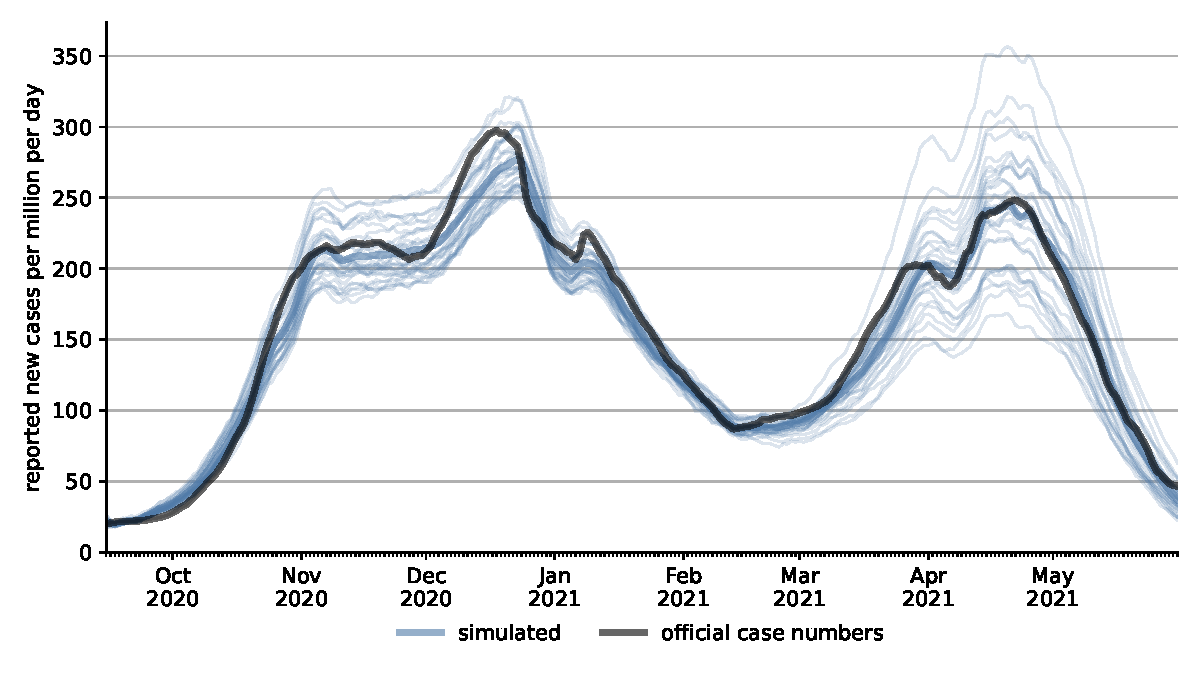
\includegraphics[width=\textwidth]{figures/results/figures/scenario_comparisons/combined_fit/full_new_known_case_with_single_runs}
    \caption{Observed Incidence in the Model and as Reported by the RKI}
    \label{fig:aggregated_fit2}
  \end{subfigure}
  \hfill
  \begin{subfigure}[b]{0.425\textwidth}
    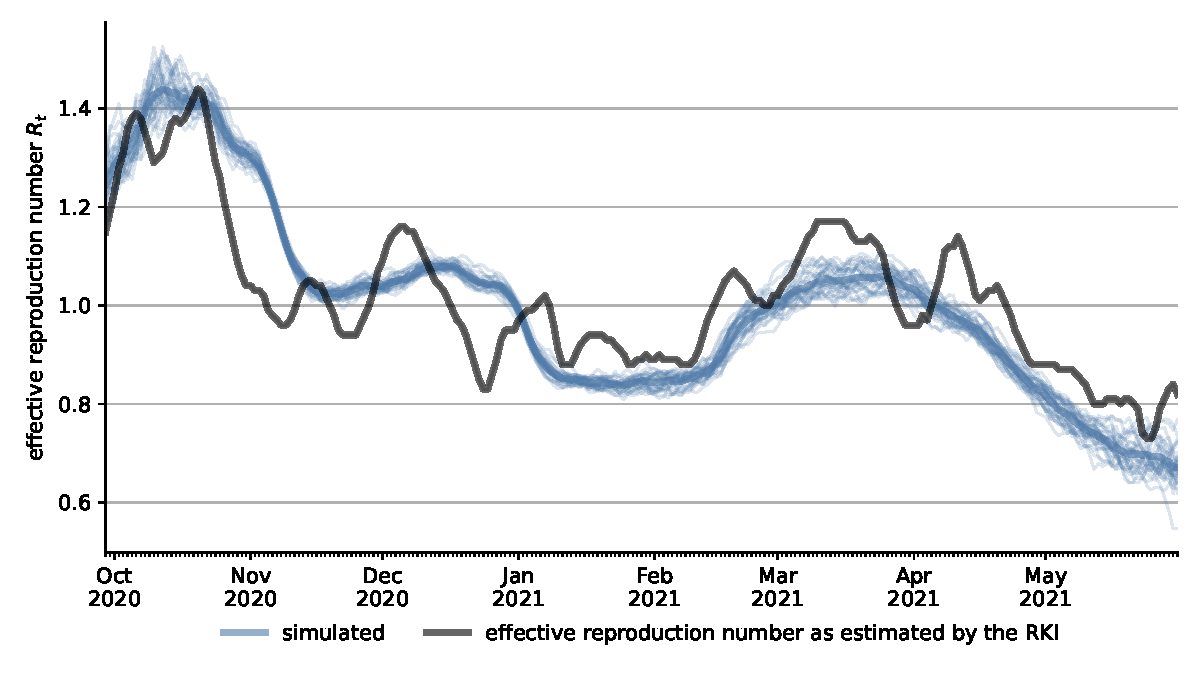
\includegraphics[width=\textwidth]{figures/results/figures/scenario_comparisons/combined_fit/full_r_effective_with_single_runs}
    \caption{Effective Replication Number $R_t$ in the Model and as Reported by the RKI}
    \label{fig:fit_r_effective}
  \end{subfigure}

  \caption{Model Fit of the Reported Cases and the Effective Replication Number}
  \label{fig:incidence_and_r_effective}

  \floatfoot{\noindent \textit{Note:} Both figures show averages and single runs. The
  average is the thick line. Single runs are shown as lighter and thinner lines. We
  averaged and show 30 simulation runs. The left figure shows the daily incidence rate
  per million for the simulated reported infection rates. The
  official case numbers as reported by the RKI are plotted in black. The fit is overall
  very good. The right figure shows the effective replication
  number ($R_t$) as reported by the RKI and as calculated in our model. The $R_t$ gives
  the average number of new infections caused by one infected individual. The $R_t$ in
  our model broadly follows the $R_t$ reported by the RKI. Two differences stand out.
  Firstly, the RKI's $R_t$ drops faster in November. This is likely due to a decline in
  the estimated overall share of detected cases ($\psi_t$) when the second wave hit
  Germany. The second difference is from mid February to mid March where the RKI's
  reported $R_t$ increased more rapidly than that in our model. Here the opposite effect
  can be expected. During this time rapid tests increased strongly leading to more cases
  being detected. In the short term this leads an $R_t$ estimation that is based on
  detected cases to overestimate the replication number.
  For legibility reasons, all lines are rolling 7-day averages.}
\end{figure}

% R effective
Our fit of the effective replication number $R_t$ closely follows the values reported by
the RKI (see Figure~\ref{fig:fit_r_effective}) even though we calculate $R_t$ on all
infected individuals not just the detected cases. This explains why the $R_t$ in our
simulations is higher during phases where the share of detected cases ($\psi_t$) falls.
This is the case in the fall of 2020 (see Figure~\ref{fig:share_known_cases_data}) where
the RKI underestimated the effective replication number due to observing a falling share
of cases. Analogously, the $R_t$ in our simulations is lower than the $R_t$ reported by
the RKI in spring where the share of known cases increased due to increased rapid
testing.

\FloatBarrier

% observed infections by age group
Zooming into the different age groups in Figure~\ref{fig:age_group_fit}, we can see that
our model is also able to reproduce the infection rates on this level. The only major
deviation from this pattern is that our model predicts too few infections for the 80 to
100 year olds. This was to be expected because our synthetic population does not include
inhabitants of nursing homes. Outbreaks in nursing homes led to a large number of
infections among the oldest during the second wave of the pandemic in Germany. Moreover,
the model predicts too few observed infections for the 15 to 34 years old at the end of
2020 and the 5 to 14 years old in April and May 2021. The former is likely due to the
fact that this age group has a very active social life which is not fully captured by our
contact networks. The latter probably comes from a too conservative model of school
reopenings.


\begin{figure}[ht]  % observed infections by age group
  \centering
  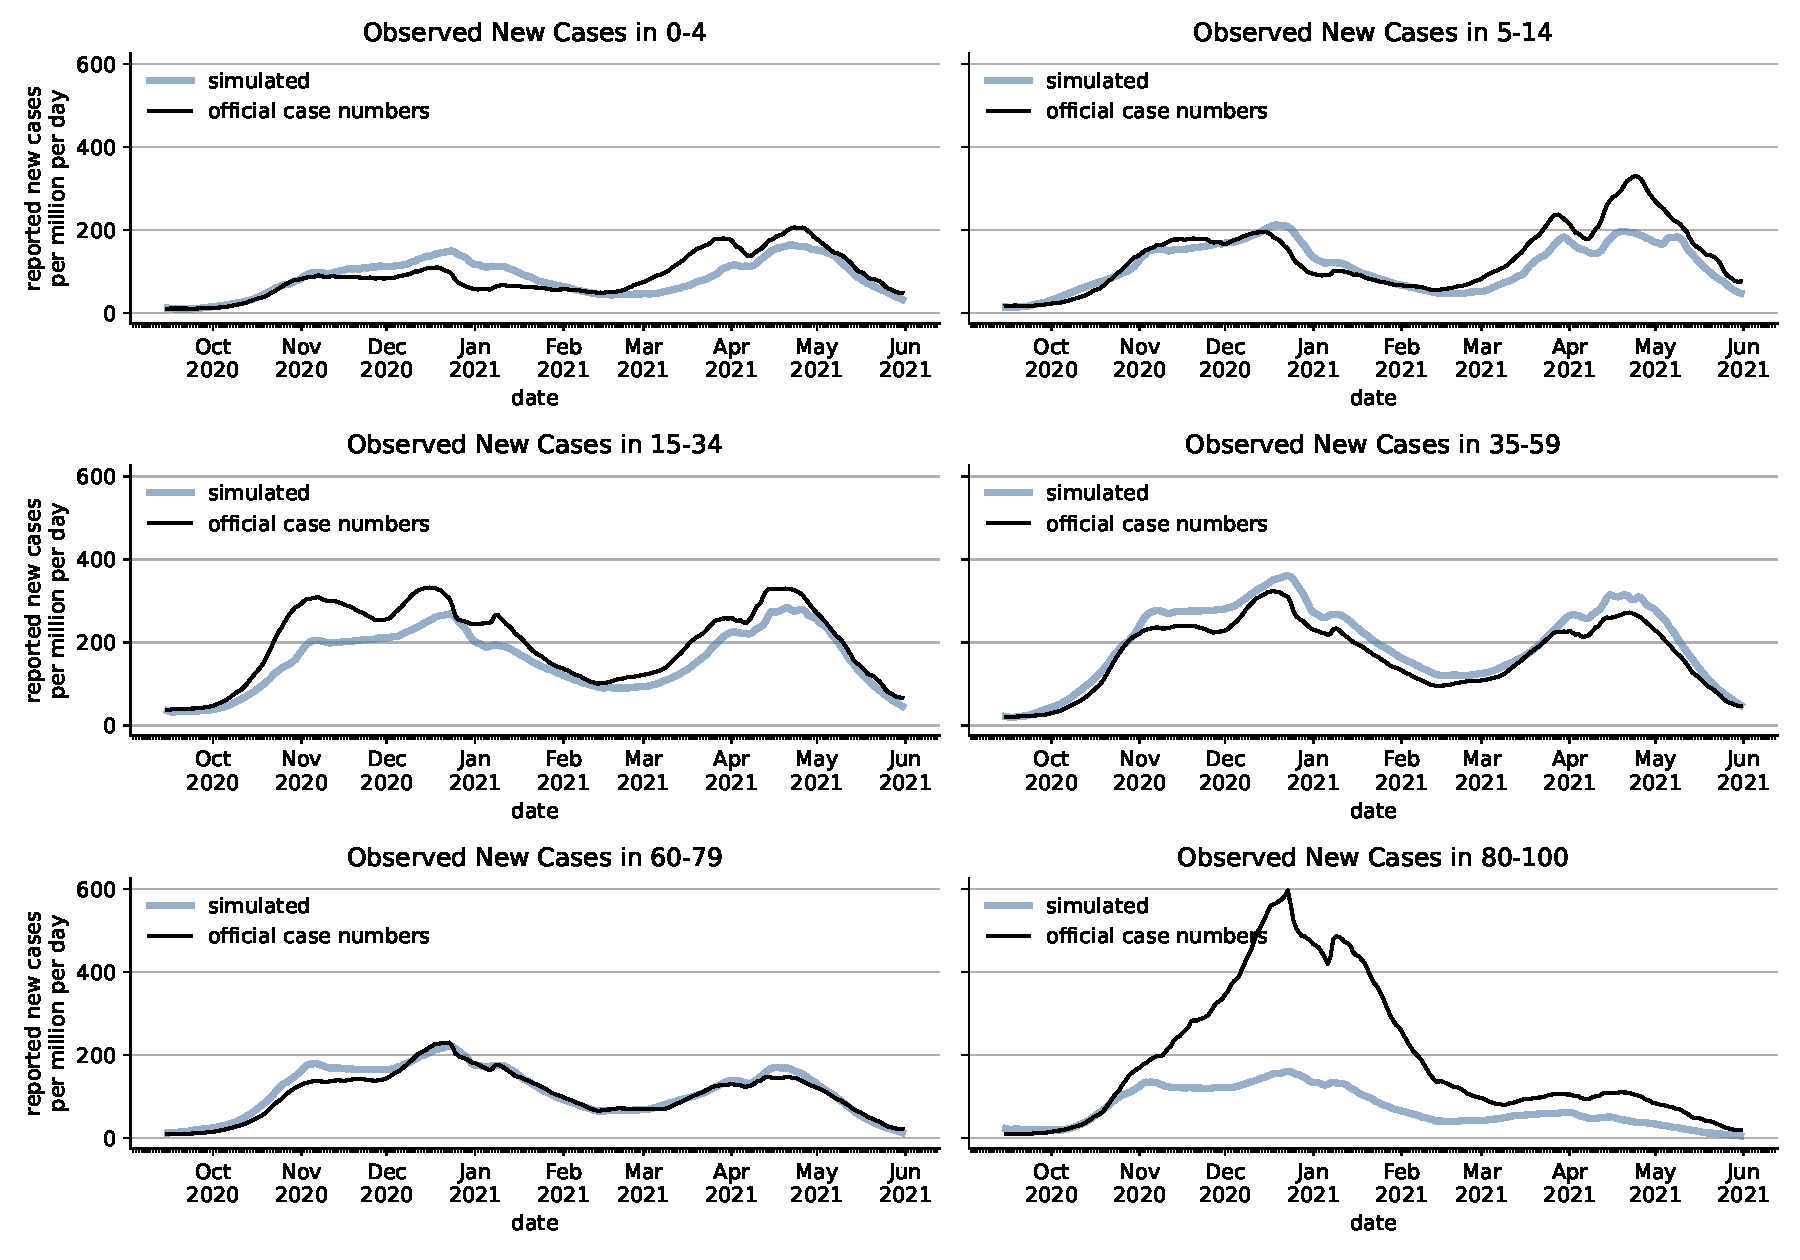
\includegraphics[width=\textwidth]{figures/results/figures/incidences_by_group/age_group_rki/full_combined_baseline_new_known_case}
  \caption{Simulated and Empirical Infections by Age Group}
  \floatfoot{\noindent \textit{Note:} The figure shows the number of reported versus
  simulated cases per one million people per day for different age groups. The age group
  of individuals above 80 needs to be interpreted with caution because our synthetic
  population only includes private households, i.e. nursing homes are not represented in
  our model. They accounted for many cases and deaths in the winter of 2020 and many 80
  to 100 year olds live in these facilities. We average over 30
  simulation runs. For legibility reasons, all lines are rolling 7-day averages.}
  \label{fig:age_group_fit}
\end{figure}


\FloatBarrier

% observed infections by federal state
Our model fit is also very good for the different German federal states. This holds not
only for the large states such as North Rhine-Westphalia or Bavaria but also for many
smaller states such as Hessen or Rhineland-Palatinate. This shows that using school
vacations dates and work mobility reductions by \cite{Google2021} at the state level
combined with county and age group specific initial conditions (see
Section~\ref{sub:initial_conditions}) and county level assortativity of contacts is
sufficient to represent many local differences.  %
The fit is especially good given that our model does not aim to have a high local
resolution. For example we abstract from population density and cross-border travel. It
is, thus, unsurprising that there are states that we do not match well, such as very
thinly populated Mecklenburg-Vorpommern and Schleswig-Holstein or Saxony with its large
border to the Czech Republic that had a much higher incidence than
Germany.

\begin{figure}[ht]   % observed infections by federal state
  \centering
  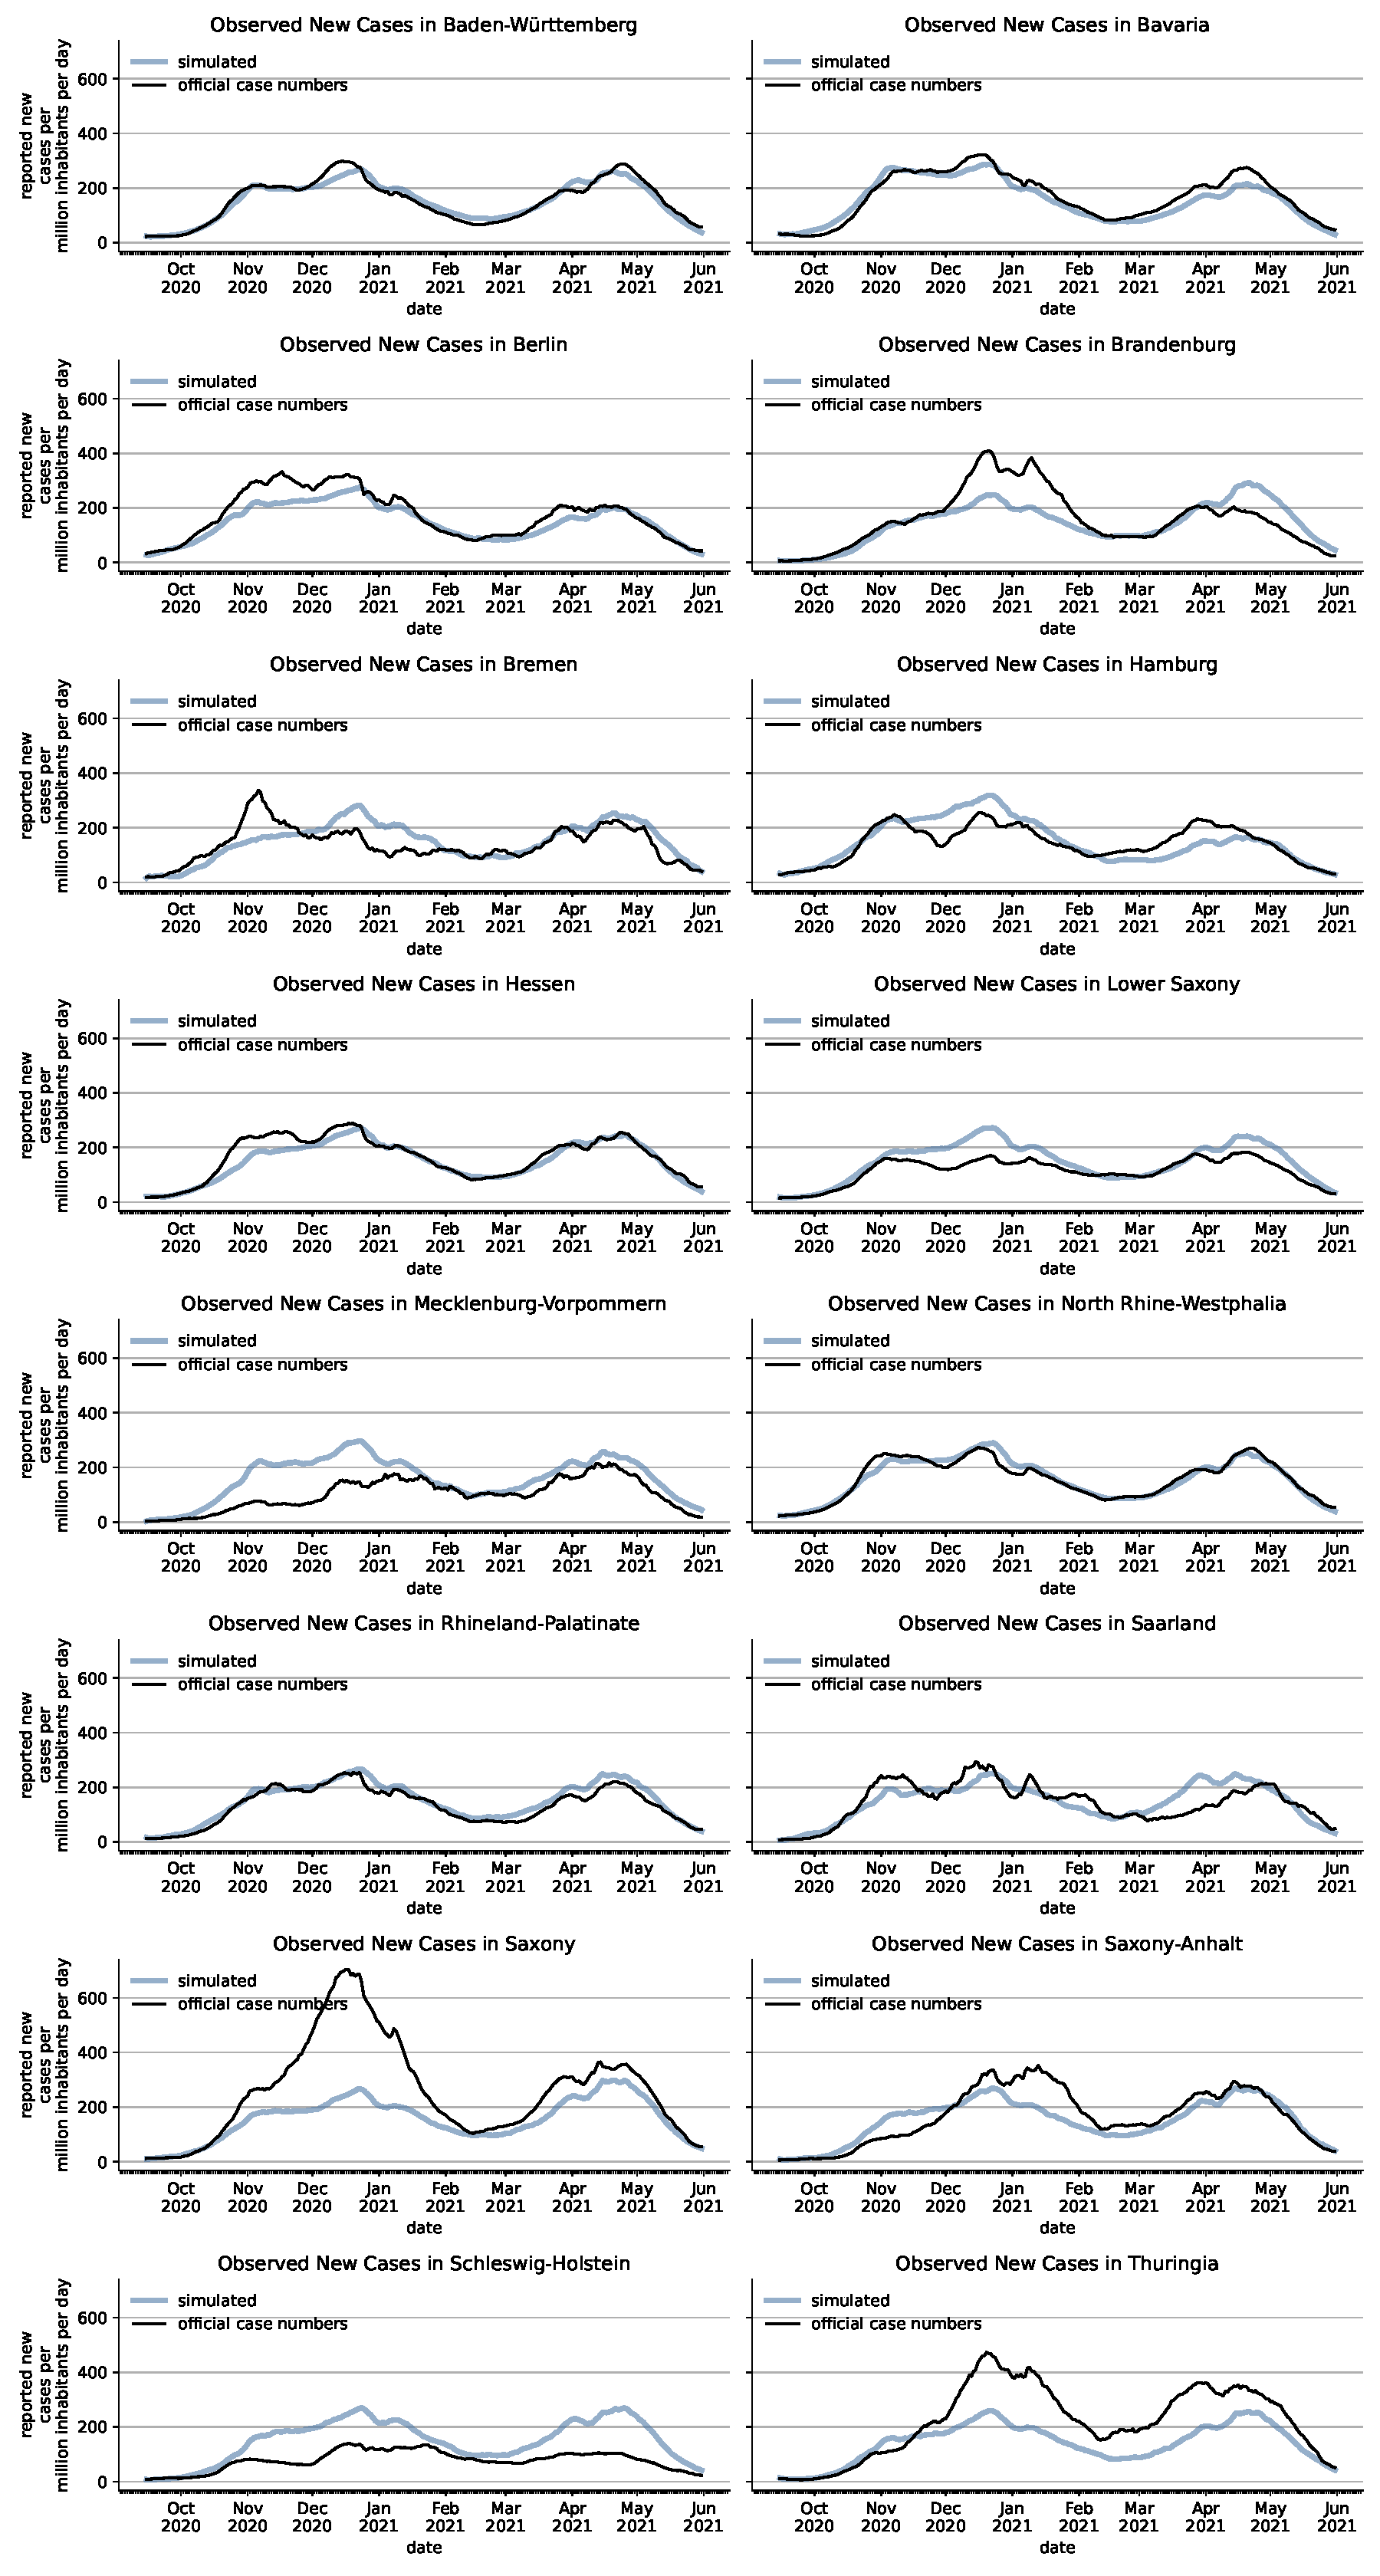
\includegraphics[height=0.95\textheight]{figures/results/figures/incidences_by_group/state/full_combined_baseline_new_known_case}
  \caption{Simulated and Empirical Infections by Federal State}
  \floatfoot{\noindent \textit{Note:} The figure shows the number of reported versus
  simulated cases per one million people per day for different federal states. We
  averaged over 30 simulation runs. For legibility reasons, all lines are rolling 7-day averages.}
  \label{fig:state_fit}
\end{figure}

\FloatBarrier

% B.1.1.7
We fit the proliferation of the B.1.1.7 variant quite exactly despite only introducing a
few cases in January ($\omega_{B.1.1.7,t}$) as can be seen in
Figure~\ref{fig:fit_share_b117}. Since we only model B.1.1.7 and do not include other
variants, B.1.1.7 reaches a share of nearly 100\% by May while the true rate plateaued at
90\%. By the end of May B.1.617.2 gained traction in Germany. However, given that
B.1.617.2 made up less than 5\% even at the end of our simulation period, we did not
include it in our model.

\begin{figure}[ht]
  \centering

  \begin{subfigure}[b]{0.425\textwidth}   % Share B.1.1.7
    \centering
    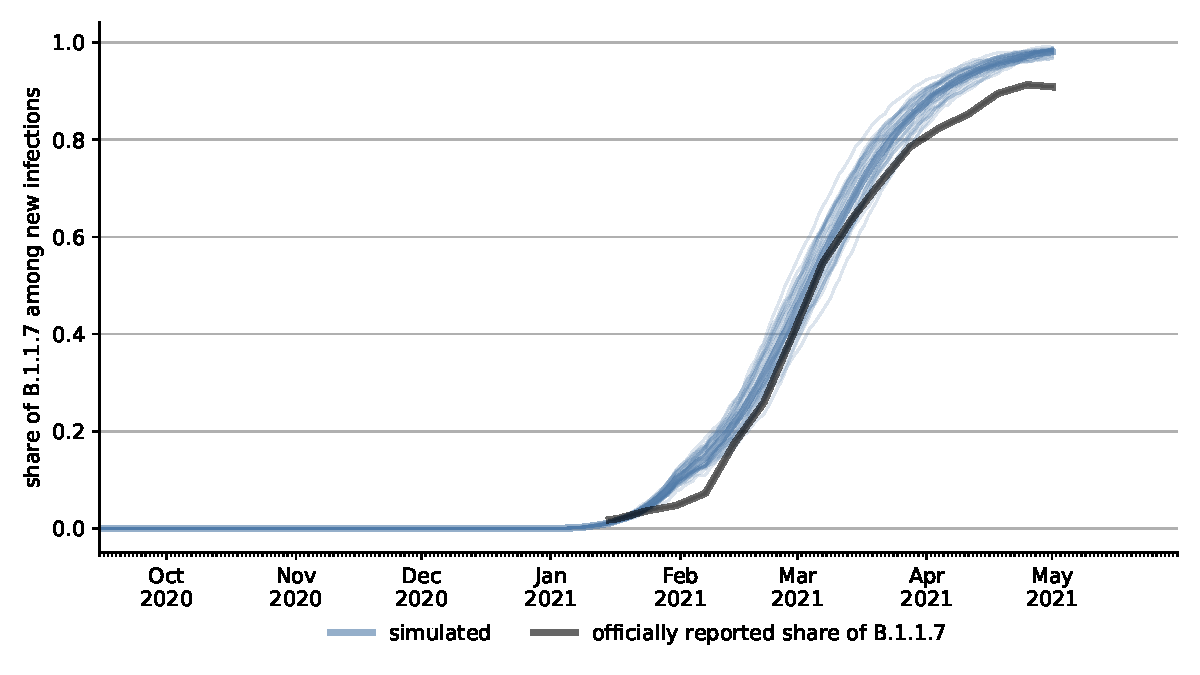
\includegraphics[width=\textwidth]{figures/results/figures/scenario_comparisons/combined_fit/full_share_b117_with_single_runs}
    \caption{Share of B.1.1.7 in the Model and as Reported by the RKI}
    \label{fig:fit_share_b117}
  \end{subfigure}
  \hfill
  \begin{subfigure}[b]{0.425\textwidth}    % Vaccinations
    \centering
    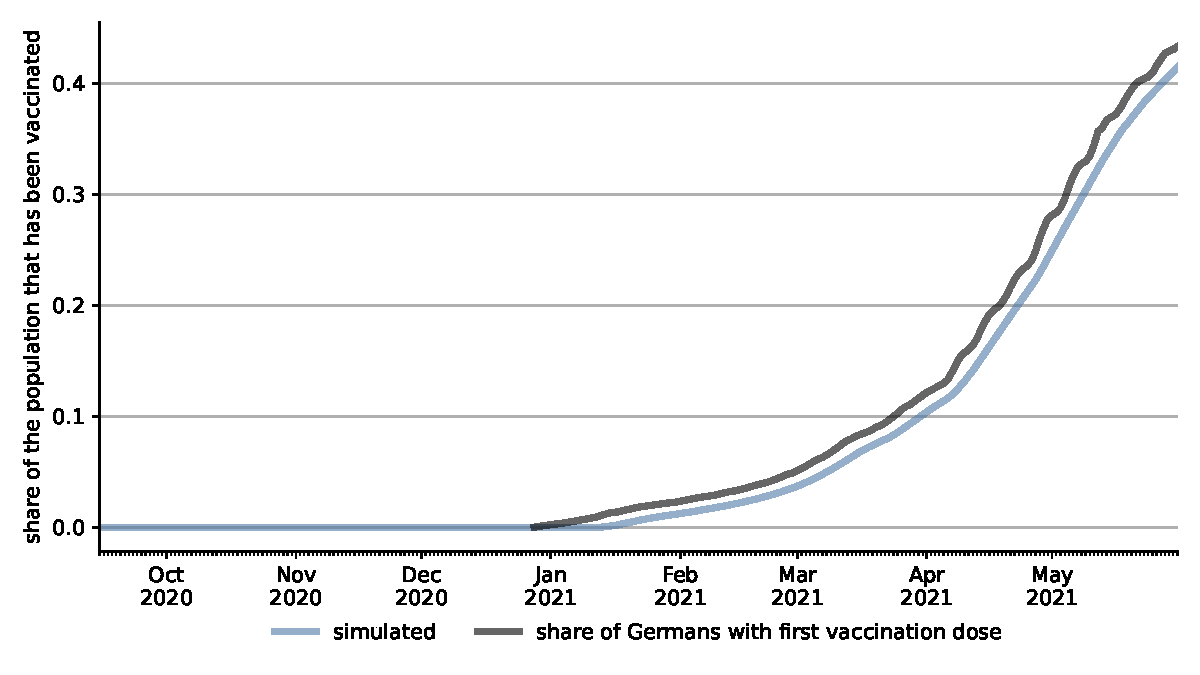
\includegraphics[width=\textwidth]{figures/results/figures/scenario_comparisons/combined_fit/full_ever_vaccinated}
    \caption{Share of Vaccinated Individuals in the Model and the German Population}
    \label{fig:fit_vaccinations}
  \end{subfigure}
  \caption{Model Fit of the Share of B.1.1.7 and Vaccinations}
  \floatfoot{\noindent \textit{Note:} The left figure shows the share of B.1.1.7 as
  reported by the RKI and as calculated in our model. We only introduce a few cases over
  the course of January. From then B.1.1.7 takes over endogenously through its increased
  infectiousness ($\sigma_{B.1.1.7}$). The right figure shows the rate
  of individuals that are vaccinated in our synthetic population versus in the general
  German population. For legibility reasons, all lines are rolling 7-day averages.}
\end{figure}

% vaccinations
The fit of the share of vaccinated individuals can be seen in
Figure~\ref{fig:fit_vaccinations}. In Germany, vaccines were rolled out according to four
priority groups. The first vaccines were mostly reserved for nursing homes and some
selected professions such as first responders. Since we do not have nursing home
inhabitants in our model, we subtract the first percent of vaccinations which is
equivalent to the share of Germans living in nursing homes. Afterwards, the share of
vaccinated individuals in the population follows the German increase exactly. We took
great care to model the prioritization of older individuals and professions that cannot
reduce physical contact easily such as teachers or medical staff (see
Section~\ref{subsec:synthetic_population} and Figure~\ref{fig:vaccinations_by_age_group}
for the vaccination rates in our model by age group).

\FloatBarrier

% rapid test demand
The most difficult moment to match in our model is the rapid test demand. This is because
we have five different channels through which individuals demand rapid tests and many of
the demand curves are at least partially calibrated through survey data. It is therefore
very reassuring that we fit the share of individuals that do weekly rapid tests almost
perfectly. For the share of individuals that have ever done a rapid test our model is
conservative. There are two reasons for this: Firstly, we do not model people who have
done rapid tests out of curiosity once they became available. Secondly, in the model, the
decision to take a rapid test is based on a time invariant individual specific compliance
factor without any additional random components. While this captures important features
of rapid test demand it abstracts from people who turn down rapid tests most of the time
but accept them sometimes. Fortunately, Section~\ref{subsec:model_validation} shows that
our main results are robust to changes in the exact shares of individuals demanding rapid
tests.

\begin{figure}[ht]     % rapid test demand
    \centering
    \label{fig:share_ever_rapid_test2}
    \begin{subfigure}{.425\textwidth}
        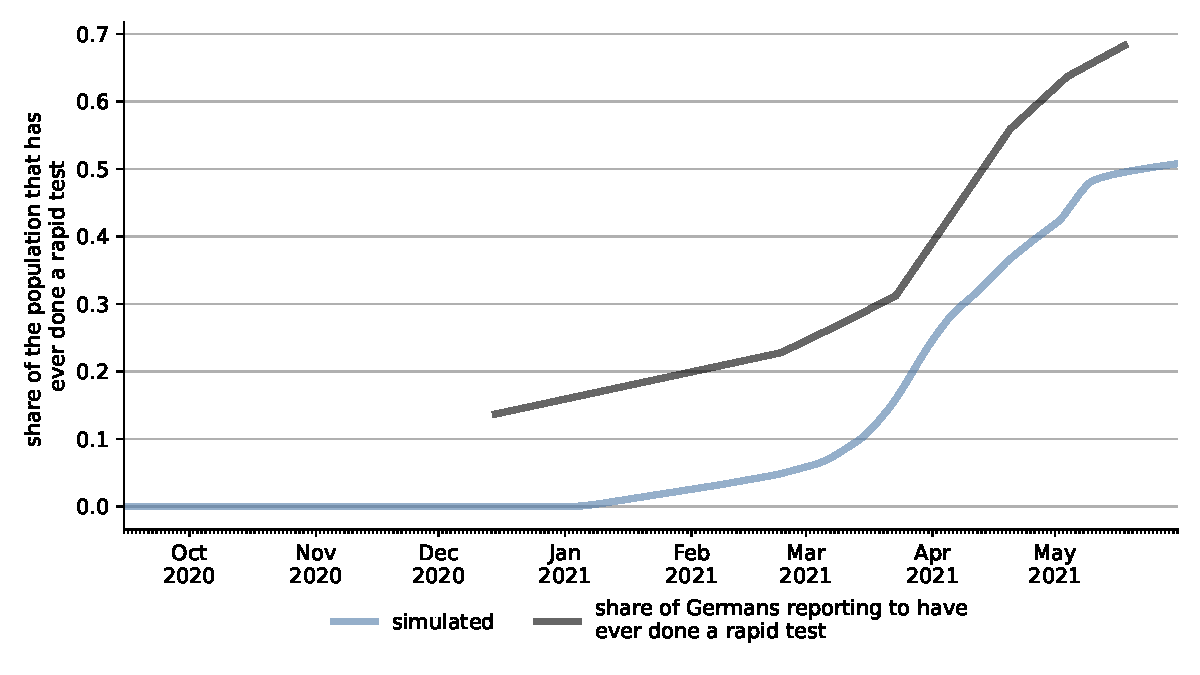
\includegraphics[width=0.9 \textwidth]{figures/results/figures/scenario_comparisons/combined_fit/full_share_ever_rapid_test}
        \caption{Share of the Population That Has Ever Done a Rapid Test}
    \end{subfigure}%
    \hfill
    \begin{subfigure}{.425\textwidth}
        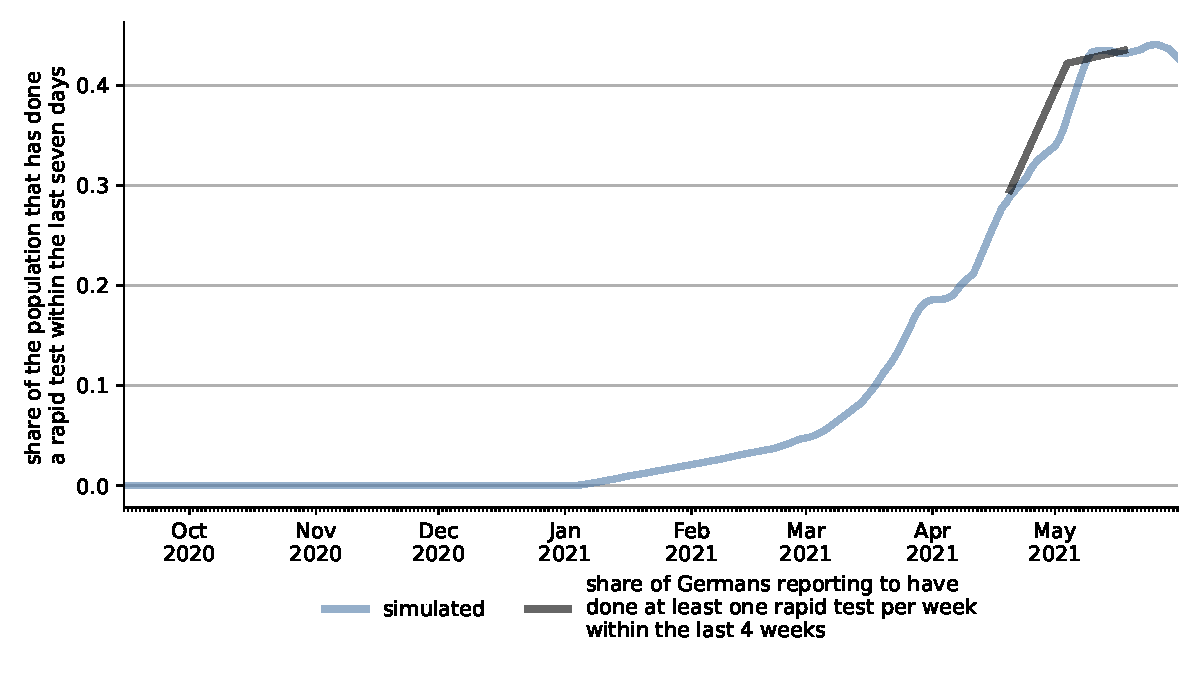
\includegraphics[width=0.9 \textwidth]{figures/results/figures/scenario_comparisons/combined_fit/full_share_rapid_test_in_last_week}
        \caption{Share of the Population That Did a Rapid Test in the Last Week}
    \end{subfigure}

    \caption{Share of Individuals With Rapid Tests}
    \label{fig:share_rapid_test_last_week2}

    \floatfoot{\noindent \textit{Note:} Both panels compare empirical and simulated
        rapid test demands. The empirical data comes from \citet{Betsch2021b}.
        The left panel compares the share of individuals who have ever done a rapid test.
        The right
        panel compares the share of individuals who have done a rapid test within the
        last seven days in our simulation compared to the share reporting to have done at
        least weekly rapid tests in the last four weeks in the COSMO survey. Overall our
        calibration of rapid tests are slightly conservative. The overall share is below
        that in the study. We fit the share of weekly tests quite exactly.
        For legibility reasons, all simulated lines are rolling 7-day averages. % However, the
        % study only covers adults while our share also includes children who are tested
        % very regularly when attending school.
      }
\end{figure}



\FloatBarrier

